\documentclass[12pt, english]{article}\usepackage[]{graphicx}\usepackage[]{xcolor}
% maxwidth is the original width if it is less than linewidth
% otherwise use linewidth (to make sure the graphics do not exceed the margin)
\makeatletter
\def\maxwidth{ %
  \ifdim\Gin@nat@width>\linewidth
    \linewidth
  \else
    \Gin@nat@width
  \fi
}
\makeatother

\definecolor{fgcolor}{rgb}{0.345, 0.345, 0.345}
\newcommand{\hlnum}[1]{\textcolor[rgb]{0.686,0.059,0.569}{#1}}%
\newcommand{\hlsng}[1]{\textcolor[rgb]{0.192,0.494,0.8}{#1}}%
\newcommand{\hlcom}[1]{\textcolor[rgb]{0.678,0.584,0.686}{\textit{#1}}}%
\newcommand{\hlopt}[1]{\textcolor[rgb]{0,0,0}{#1}}%
\newcommand{\hldef}[1]{\textcolor[rgb]{0.345,0.345,0.345}{#1}}%
\newcommand{\hlkwa}[1]{\textcolor[rgb]{0.161,0.373,0.58}{\textbf{#1}}}%
\newcommand{\hlkwb}[1]{\textcolor[rgb]{0.69,0.353,0.396}{#1}}%
\newcommand{\hlkwc}[1]{\textcolor[rgb]{0.333,0.667,0.333}{#1}}%
\newcommand{\hlkwd}[1]{\textcolor[rgb]{0.737,0.353,0.396}{\textbf{#1}}}%
\let\hlipl\hlkwb

\usepackage{framed}
\makeatletter
\newenvironment{kframe}{%
 \def\at@end@of@kframe{}%
 \ifinner\ifhmode%
  \def\at@end@of@kframe{\end{minipage}}%
  \begin{minipage}{\columnwidth}%
 \fi\fi%
 \def\FrameCommand##1{\hskip\@totalleftmargin \hskip-\fboxsep
 \colorbox{shadecolor}{##1}\hskip-\fboxsep
     % There is no \\@totalrightmargin, so:
     \hskip-\linewidth \hskip-\@totalleftmargin \hskip\columnwidth}%
 \MakeFramed {\advance\hsize-\width
   \@totalleftmargin\z@ \linewidth\hsize
   \@setminipage}}%
 {\par\unskip\endMakeFramed%
 \at@end@of@kframe}
\makeatother

\definecolor{shadecolor}{rgb}{.97, .97, .97}
\definecolor{messagecolor}{rgb}{0, 0, 0}
\definecolor{warningcolor}{rgb}{1, 0, 1}
\definecolor{errorcolor}{rgb}{1, 0, 0}
\newenvironment{knitrout}{}{} % an empty environment to be redefined in TeX

\usepackage{alltt}
\usepackage{mypreamble, myRpreamble}
\IfFileExists{upquote.sty}{\usepackage{upquote}}{}
\begin{document}
{\bf Arkaraj Mukherjee \\ Homework 11}
\begin{knitrout}
\definecolor{shadecolor}{rgb}{0.969, 0.969, 0.969}\color{fgcolor}\begin{kframe}
\begin{alltt}
\hlkwd{library}\hldef{(tidyverse);}
\end{alltt}


{\ttfamily\noindent\itshape\color{messagecolor}{\#\# -- Attaching core tidyverse packages ---------------------------------------- tidyverse 2.0.0 --\\\#\# v dplyr \ \ \ \ 1.2.0 \ \ \ \ v readr \ \ \ \ 2.1.6\\\#\# v forcats \ \ 1.0.1 \ \ \ \ v stringr \ \ 1.6.0\\\#\# v ggplot2 \ \ 4.0.2 \ \ \ \ v tibble \ \ \ 3.3.1\\\#\# v lubridate 1.9.5 \ \ \ \ v tidyr \ \ \ \ 1.3.2\\\#\# v purrr \ \ \ \ 1.2.1 \ \ \ \ \\\#\# -- Conflicts ---------------------------------------------------------- tidyverse\_conflicts() --\\\#\# x dplyr::filter() masks stats::filter()\\\#\# x dplyr::lag() \ \ \ masks stats::lag()\\\#\# i Use the conflicted package (<http://conflicted.r-lib.org/>) to force all conflicts to become errors}}\begin{alltt}
\hlkwd{set.seed}\hldef{(}\hlnum{123}\hldef{);}
\end{alltt}
\end{kframe}
\end{knitrout}

\begin{enumerate}[label=\arabic*.]
\item	
	\begin{enumerate}[label=(\alph*)]
	\item Since $H_1 : m > m_0$, large values of the sign statistic $S = \#\{i : X_i > m_0\}$ favor the alternative.
	Under $H_0$, we have $S \sim \mathrm{Binomial}(n, \tfrac{1}{2})$ so the rejection region at level $\alpha$ is
	\[
    	S \geq b^*, \quad \text{where } b^* = \min\left\{ b : \sum_{k=b}^{n} \binom{n}{k} \left(\tfrac{1}{2}\right)^n \leq \alpha \right\}.
	\]
	\item Since $H_1 : m < m_0$, small values of the sign statistic $S = \#\{i : X_i > m_0\}$ favor the alternative.
	Under $H_0$, we have $S \sim \mathrm{Binomial}(n, \tfrac{1}{2})$, so the rejection region at level $\alpha$ is
	\[
	    S \leq b_*, \quad \text{where } b_* = \max\left\{ b : \sum_{k=0}^{b} \binom{n}{k} \left(\tfrac{1}{2}\right)^n \leq \alpha \right\}.
	\]
	\end{enumerate}
\item 
	\begin{enumerate}[label=(\alph*)]
		\item This is false, $U$ in definition $1$ is $U_2$ as in definition $3$. Suppose we have $Y_{i_1}\leq\ldots\leq Y_{i_m}$ (i.e. $Y_{i_k}$ is the sample with rank $k$) and let $r_k$ be the rank of $Y_{i_k}$ in the entire data set, then we clearly see that there are exactly $k-1$ $Y_i$'s less than or equal to $Y_{i_k}$ and thus exactly $r_k-1-(k-1)=r_k-k$ $Y_i$'s less than or equal to $X_{i_k}$, thus we see that the presence of $X_{i_k}$ contributes exaclty $r_k-k$ to $U$ so we have $U=\sum_{k=m}^nr_k-k=W_2-m(m+1)/2=U_2$ where $W_2$ is as defined in definition $3$ and so is $U_2$ and we also thus see that, (as per definition $3$ for everything other than $U$) $P(W_2\leq w)=P(U+m(m+1)/2\leq w)=P(U\leq w-n(n+1)/2)$ so $C_1=m(m+1)/2.$ 
			However, if $X$ and $Y$ were replaced in definition $1$ then the claim would hold.
		\item $W_1+W_2$ is the sum of all the ranks and is equal to $(n+m)(n+m+1)2$ and thus, $U_1+U_2=(n+m)(n+m+1)/2-n(n+1)/2-m(m+1)/2=nm$. 
			Thus, $P(U_2\leq u_2)=P(nm-U_1\leq u_2)=P(U_1\geq nm-u_2)$ so we have $C_2=nm.$
		\item This is false as per definition $3$ (it is not mentioned which definition we have used so we go with $3$ as otherwise the $U$ defined in it would be redundant otherwise)
			We demonstrate this statistically below 
\begin{knitrout}
\definecolor{shadecolor}{rgb}{0.969, 0.969, 0.969}\color{fgcolor}\begin{kframe}
\begin{alltt}
\hldef{experiment} \hlkwb{=} \hlkwa{function}\hldef{(}\hlkwc{num_sim}\hldef{,}\hlkwc{n}\hldef{,}\hlkwc{m}\hldef{,}\hlkwc{u_1}\hldef{,}\hlkwc{sampling_dist}\hldef{) \{}
\hldef{u_2} \hlkwb{=} \hldef{n}\hlopt{*}\hldef{m} \hlopt{-} \hldef{u_1}
\hlcom{#calculating empirical probability of LHS under null hypothesis}
\hlcom{#where X,Y have the same dist., say its standard normal}
\hldef{indicator_vec} \hlkwb{=} \hlkwd{replicate}\hldef{(num_sim,}
\hldef{\{}
\hldef{X}\hlkwb{=}\hlkwd{sampling_dist}\hldef{(n)}
\hldef{Y}\hlkwb{=}\hlkwd{sampling_dist}\hldef{(m)}
\hldef{comb} \hlkwb{=} \hlkwd{c}\hldef{(X,Y)}
\hldef{ranks} \hlkwb{=} \hlkwd{rank}\hldef{(comb)}
\hldef{W_1} \hlkwb{=} \hlkwd{sum}\hldef{(ranks[}\hlnum{1}\hlopt{:}\hldef{n])}
\hldef{W_2} \hlkwb{=} \hlkwd{sum}\hldef{(ranks[(n}\hlopt{+}\hlnum{1}\hldef{)}\hlopt{:}\hldef{(n}\hlopt{+}\hldef{m)])}
\hldef{U_1} \hlkwb{=} \hldef{W_1} \hlopt{-} \hldef{n}\hlopt{*}\hldef{(n}\hlopt{+}\hlnum{1}\hldef{)}\hlopt{/}\hlnum{2}
\hldef{U_2} \hlkwb{=} \hldef{W_2} \hlopt{-} \hldef{m}\hlopt{*}\hldef{(m}\hlopt{+}\hlnum{1}\hldef{)}\hlopt{/}\hlnum{2}
\hldef{U} \hlkwb{=} \hlkwd{min}\hldef{(U_1,U_2)}
\hlkwd{as.numeric}\hldef{(}\hlkwd{c}\hldef{(U_1} \hlopt{<=} \hldef{u_1, U_1} \hlopt{>=} \hldef{u_1, U} \hlopt{<=} \hlkwd{min}\hldef{(u_1,u_2)))}
\hldef{\})}
\hlcom{#this is a 3x10^5 matrix}
\hldef{results} \hlkwb{=} \hlkwd{rowMeans}\hldef{(indicator_vec)}
\hldef{LHS} \hlkwb{=} \hlkwd{min}\hldef{(results[}\hlnum{1}\hlopt{:}\hlnum{2}\hldef{])}
\hldef{RHS} \hlkwb{=} \hldef{results[}\hlnum{3}\hldef{]}
\hlkwd{c}\hldef{(LHS,RHS)}
\hldef{\}}
\hlcom{#u_1 is atmost (m+1)+...+(m+n)-n(n+1)/2 = nm}
\hldef{v_1}\hlkwb{=}\hlkwd{experiment}\hldef{(}\hlnum{10}\hlopt{^}\hlnum{5}\hldef{,}\hlnum{30}\hldef{,}\hlnum{40}\hldef{,}\hlnum{467}\hldef{,rnorm)}
\hldef{v_2}\hlkwb{=}\hlkwd{experiment}\hldef{(}\hlnum{10}\hlopt{^}\hlnum{5}\hldef{,}\hlnum{10}\hldef{,}\hlnum{20}\hldef{,}\hlnum{100}\hldef{,rnorm)}
\hlcom{# \textbackslash{}(x) f(x,...) is basically treated as g(x):=f(x,...)}
\hldef{v_3}\hlkwb{=}\hlkwd{experiment}\hldef{(}\hlnum{10}\hlopt{^}\hlnum{5}\hldef{,}\hlnum{1200}\hldef{,}\hlnum{300}\hldef{,}\hlnum{170000}\hldef{,\textbackslash{}(}\hlkwc{n}\hldef{)} \hlkwd{rpois}\hldef{(n,}\hlkwc{lambda}\hldef{=}\hlnum{4}\hldef{))}
\hldef{temp} \hlkwb{=} \hlkwa{function}\hldef{(}\hlkwc{v}\hldef{) \{v[}\hlnum{1}\hldef{]}\hlopt{/}\hldef{v[}\hlnum{2}\hldef{]\}}
\hlkwd{temp}\hldef{(v_1)}
\end{alltt}
\begin{verbatim}
## [1] 0.5032572
\end{verbatim}
\begin{alltt}
\hlkwd{temp}\hldef{(v_2)}
\end{alltt}
\begin{verbatim}
## [1] 0.50813
\end{verbatim}
\begin{alltt}
\hlkwd{temp}\hldef{(v_3)}
\end{alltt}
\begin{verbatim}
## [1] 0.4958072
\end{verbatim}
\end{kframe}
\end{knitrout}
			We can safely conclude that this is false, but the experiment suggests that $2\times\texttt{LHS}= \texttt{RHS}$, this can be proved to be true when we sample from continuous distributions but it still fails for small discrete cases so theres no saving this.		
	\end{enumerate}
\item
	\begin{enumerate}[label=(\alph*)]
	\item
\begin{knitrout}
\definecolor{shadecolor}{rgb}{0.969, 0.969, 0.969}\color{fgcolor}\begin{kframe}
\begin{alltt}
\hldef{dat} \hlkwb{=} \hlkwd{read.csv}\hldef{(}\hlsng{"scores.csv"}\hldef{)}
\hlkwd{head}\hldef{(dat)}
\end{alltt}
\begin{verbatim}
##   Entrance UG
## 1      756 85
## 2      815 91
## 3      828 57
## 4      690 18
## 5      911 58
## 6      581 43
\end{verbatim}
\begin{alltt}
\hldef{rho} \hlkwb{=} \hlkwd{cor}\hldef{(dat}\hlopt{$}\hldef{Entrance,dat}\hlopt{$}\hldef{UG)}
\hldef{rho}
\end{alltt}
\begin{verbatim}
## [1] 0.2944079
\end{verbatim}
\end{kframe}
\end{knitrout}
	\item (and (c) as instructed)
\begin{knitrout}
\definecolor{shadecolor}{rgb}{0.969, 0.969, 0.969}\color{fgcolor}\begin{kframe}
\begin{alltt}
\hlcom{# b}
\hldef{n} \hlkwb{=} \hlkwd{length}\hldef{(dat}\hlopt{$}\hldef{UG)}
\hldef{cor_boot_est}\hlkwb{=}\hlkwd{replicate}\hldef{(}\hlnum{1000}\hldef{,\{}
\hldef{s} \hlkwb{=} \hlkwd{sample}\hldef{(}\hlnum{1}\hlopt{:}\hldef{n,n,}\hlkwc{replace}\hldef{=}\hlnum{TRUE}\hldef{)}
\hlkwd{cor}\hldef{(dat}\hlopt{$}\hldef{Entrance[s],dat}\hlopt{$}\hldef{UG[s])}
\hldef{\})}
\hlkwd{hist}\hldef{(cor_boot_est)}
\end{alltt}
\end{kframe}
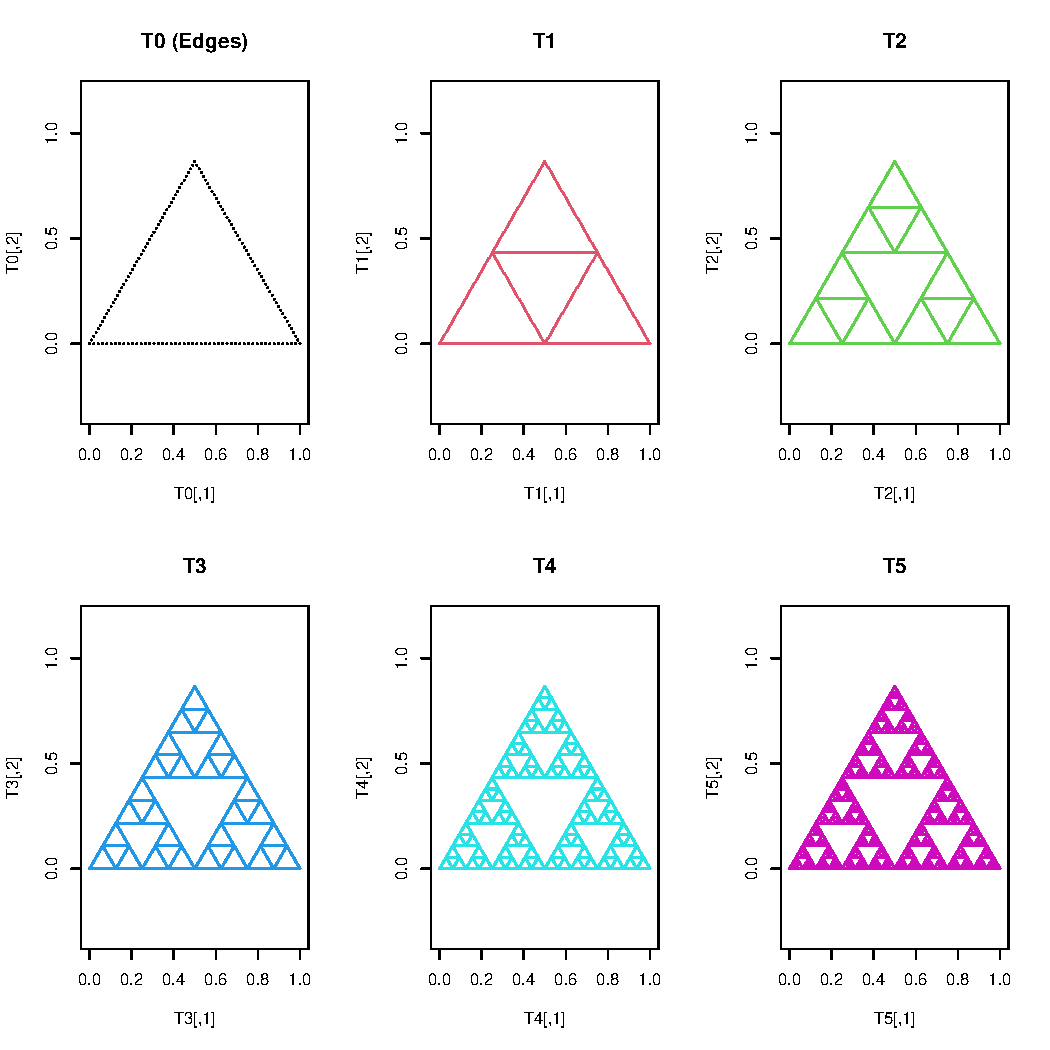
\includegraphics[width=\maxwidth]{figure/unnamed-chunk-4-1} 
\begin{kframe}\begin{alltt}
 \hlcom{# c.(i)}
 \hldef{cor_boot_bias} \hlkwb{=} \hlkwd{mean}\hldef{(cor_boot_est)} \hlopt{-} \hldef{rho}
 \hldef{cor_boot_bias}
\end{alltt}
\begin{verbatim}
## [1] -0.001435587
\end{verbatim}
\begin{alltt}
 \hldef{cor_boot_se} \hlkwb{=} \hlkwd{sd}\hldef{(cor_boot_est)}
 \hldef{cor_boot_se}
\end{alltt}
\begin{verbatim}
## [1] 0.1507458
\end{verbatim}
\begin{alltt}
 \hlcom{# c.(ii)}
 \hldef{cor_boot_ci} \hlkwb{=} \hlkwd{as.vector}\hldef{(}\hlkwd{quantile}\hldef{(cor_boot_est,} \hlkwc{probs} \hldef{=} \hlkwd{c}\hldef{(}\hlnum{0.025}\hldef{,}\hlnum{0.975}\hldef{)))}
 \hldef{cor_boot_ci}
\end{alltt}
\begin{verbatim}
## [1] -0.02726172  0.54141480
\end{verbatim}
\begin{alltt}
 \hlcom{# c.(iii)}
 \hldef{cor_boot_pi} \hlkwb{=} \hlnum{2}\hlopt{*}\hlkwd{c}\hldef{(rho,rho)} \hlopt{-} \hlkwd{as.vector}\hldef{(}\hlkwd{quantile}\hldef{(cor_boot_est,}
 \hlkwc{probs} \hldef{=} \hlkwd{c}\hldef{(}\hlnum{0.975}\hldef{,}\hlnum{0.025}\hldef{)))}
 \hldef{cor_boot_pi}
\end{alltt}
\begin{verbatim}
## [1] 0.04740092 0.61607745
\end{verbatim}
\end{kframe}
\end{knitrout}
	\item
\begin{knitrout}
\definecolor{shadecolor}{rgb}{0.969, 0.969, 0.969}\color{fgcolor}\begin{kframe}
\begin{alltt}
\hldef{cor_jack_est} \hlkwb{=} \hlkwd{vector}\hldef{(}\hlkwc{mode} \hldef{=} \hlsng{"numeric"}\hldef{,} \hlkwc{length} \hldef{= n)}
\hlkwa{for}\hldef{(i} \hlkwa{in} \hlnum{1}\hlopt{:}\hldef{n) cor_jack_est[i]} \hlkwb{=} \hlkwd{cor}\hldef{(dat}\hlopt{$}\hldef{Entrance[}\hlopt{-}\hldef{i],dat}\hlopt{$}\hldef{UG[}\hlopt{-}\hldef{i])}
\hlkwd{hist}\hldef{(cor_jack_est)}
\end{alltt}
\end{kframe}
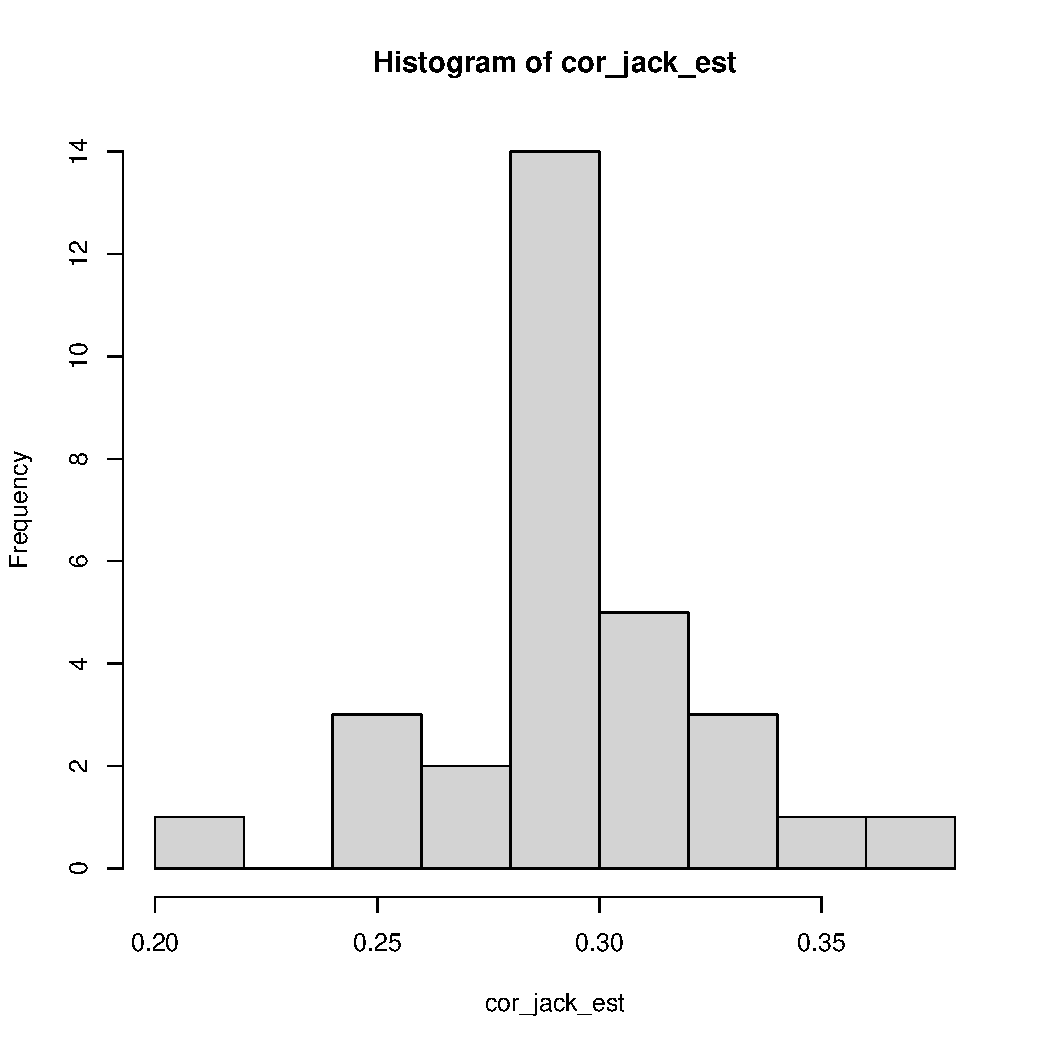
\includegraphics[width=\maxwidth]{figure/unnamed-chunk-5-1} 
\begin{kframe}\begin{alltt}
\hldef{cor_jack_bias} \hlkwb{=} \hldef{(n}\hlopt{-}\hlnum{1}\hldef{)}\hlopt{*}\hldef{(}\hlkwd{mean}\hldef{(cor_jack_est)}\hlopt{-}\hldef{rho)}
\hldef{cor_jack_bias}
\end{alltt}
\begin{verbatim}
## [1] -0.003631554
\end{verbatim}
\begin{alltt}
\hldef{cor_jack_se} \hlkwb{=} \hldef{((n}\hlopt{-}\hlnum{1}\hldef{)}\hlopt{/}\hlkwd{sqrt}\hldef{(n))}\hlopt{*}\hlkwd{sd}\hldef{(cor_jack_est)}
\hldef{cor_jack_se}
\end{alltt}
\begin{verbatim}
## [1] 0.155679
\end{verbatim}
\end{kframe}
\end{knitrout}
	
	\end{enumerate}
\end{enumerate}
\end{document}
